%%%%%%%%%%%%%%%%%%%%%%%%%%%%%%%%%%%%%%%%%%%%%%%%%%%%%%%%%%%%%%%%%%%%%%%%
\chapter{Results} \label{chap:Results}
%%%%%%%%%%%%%%%%%%%%%%%%%%%%%%%%%%%%%%%%%%%%%%%%%%%%%%%%%%%%%%%%%%%%%%%%
\vspace{1cm}

In this chapter are exposed the main results obtained from the experiments described in Chapter \ref{chap:Methods}. The analysis focuses on comparing the performance of the three investigated models, which differ in their data augmentation (DA) strategies: the nnU-Net default DA (baseline), the GIN-IPA augmentation, and a combination of both.

First, is reported the overall performance of the models across datasets---Kispi-mial, Kispi-irtk and dHCP---and labels---cerebrospinal fluid (CSF), cortical gray matter (cGM), white matter (WM), ventricles, cerebellum, deep gray matter (dGM) and brainstem (BS). Then, a pairwise comparison between models is presented, supported by statistical analyses to assess the significance and magnitude of performance differences. Finally, the robustness of the models is evaluated in a pathology-stratified analysis in the Kispi datasets.

\section{General Performance} \label{sec:GeneralPerformance}
In the plots below is shown the Dice score (DSC) across datasets and labels for the three models. Each model inference is realized on the test set of the same dataset the model was trained on (in-domain), and on the whole set (both train and test) of the other datasets (out-of-domain, OOD). Given that the general performance of the models is well captured with the DSC, here only the plots related to this metric are shown. The plots of the volume similarity (VS) and the Hausdorff distance 95\th percentile (HD95) are in Appendix \hyperref[app:SupplementaryPlots]{A}.

For the baseline model (see Fig.\,\ref{fig:default_DC}), the drop in performance between in-domain and OOD is clear in every case, except in the DSC of some labels (CSF, cGM, WM and cerebellum) for the model trained on Kispi-mial. The drop is especially evident for the models trained on the Kispi datasets when applied to dHCP. Ventricles are the most affected, but also dGM and WM. However, the change of domain does not have the same effect on the network trained on Kispi-mial as it has on the other two: for example, we have unusual high DSC values OOD for cerebellum and BS, and even higher values OOD than ID, but limited to the inference on Kispi-irtk for CSF and cGM. This is probably due to the quality of the images in Kispi-mial, which is worse than the others\,\cite{FeTA2021_review}.

\begin{figure}[htbp]
  \centering
  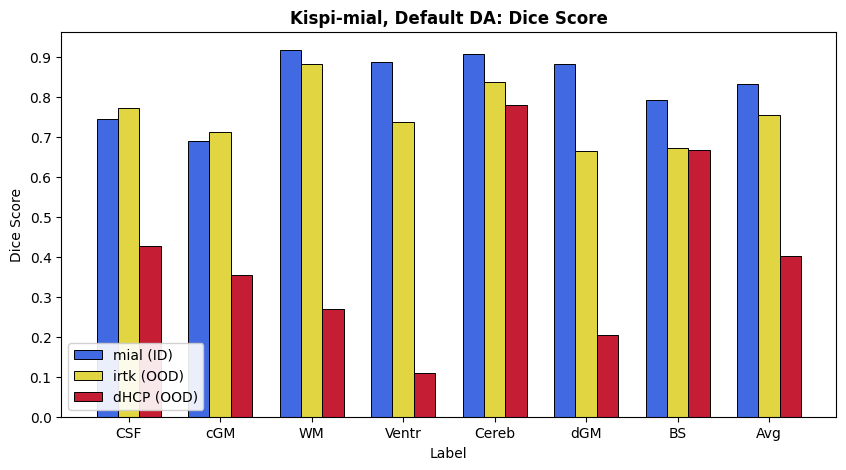
\includegraphics[width=0.8\textwidth]{figures/mial_default_DC.png} \\
  \vspace{10pt}
  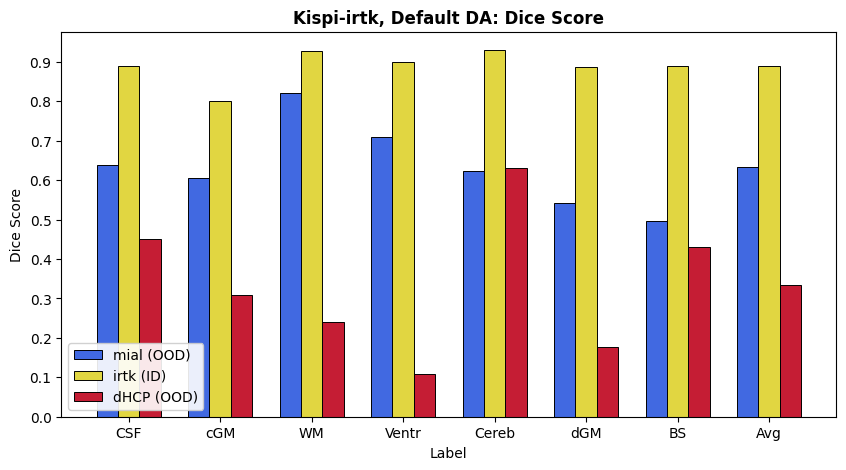
\includegraphics[width=0.8\textwidth]{figures/irtk_default_DC.png} \\
  \vspace{10pt}
  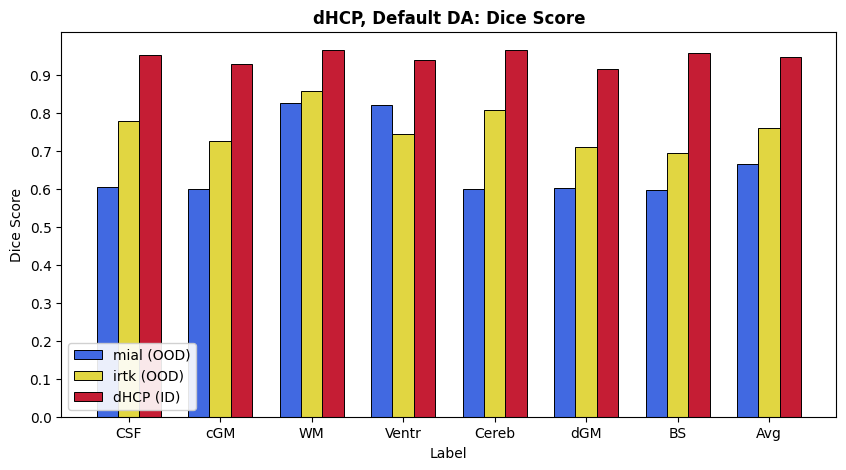
\includegraphics[width=0.8\textwidth]{figures/dHCP_default_DC.png}
  \caption{Dice score across datasets and labels for the nnU-Net default DA (baseline model). From top to bottom: training on Kispi-mial, on Kispi-irtk, and on dHCP.}
  \label{fig:default_DC}
\end{figure}

Although GIN-IPA (see Fig.\,\ref{fig:ginipa_DC}) does not cause an increment in DSC in the models trained on Kispi-mial and dHCP, it produces a significant improvement in the model trained on Kispi-irtk when predicting on dHCP. The raise is mainly located in dGM, ventricles and BS. The average Dice passes from \numrange[range-open-phrase=from\ ]{0.34}{0.54} (\qty{+58}{\percent}).

\begin{figure}[htbp]
  \centering
  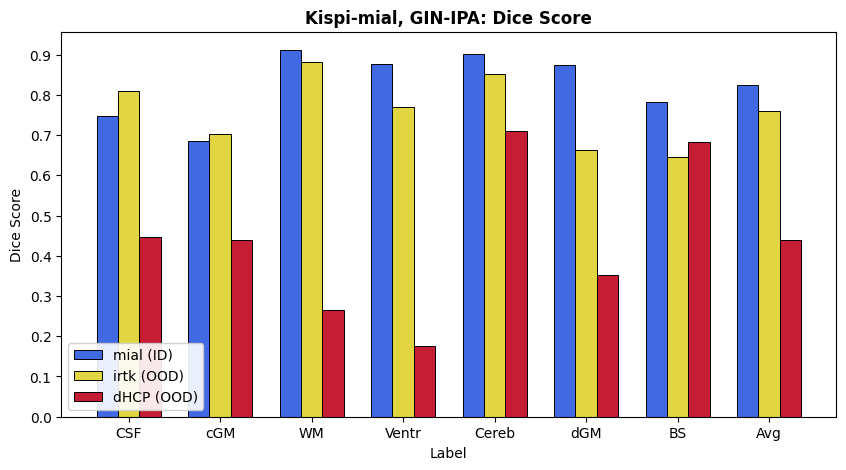
\includegraphics[width=0.8\textwidth]{figures/mial_ginipa_DC.png} \\
  \vspace{10pt}
  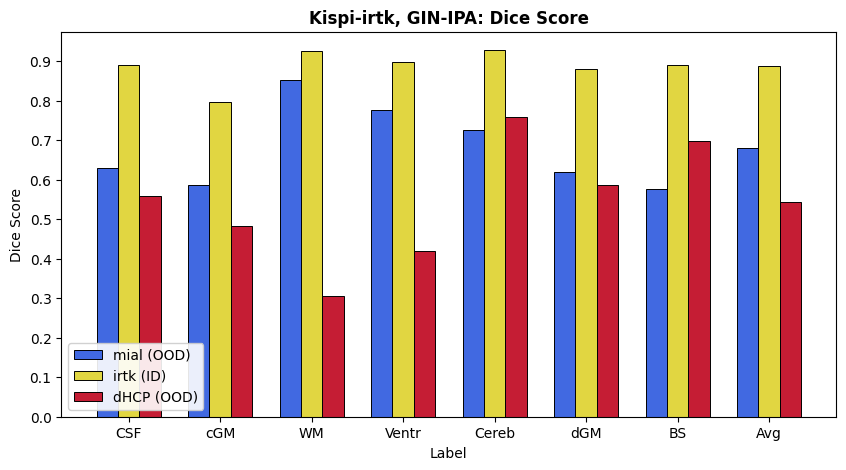
\includegraphics[width=0.8\textwidth]{figures/irtk_ginipa_DC.png} \\
  \vspace{10pt}
  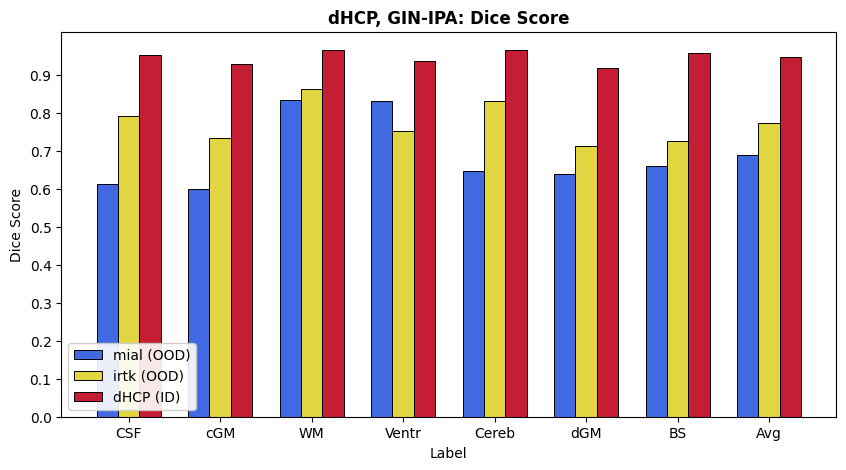
\includegraphics[width=0.8\textwidth]{figures/dHCP_ginipa_DC.png}
  \caption{Dice score across datasets and labels for the GIN-IPA DA model. From top to bottom: training on Kispi-mial, on Kispi-irtk, and on dHCP.}
  \label{fig:ginipa_DC}
\end{figure}

Finally, the model that combines the nnU-Net default DA and GIN-IPA is substantially equivalent to the pure GIN-IPA model (see Fig.\,\ref{fig:both_DC}).

\begin{figure}[htbp]
  \centering
  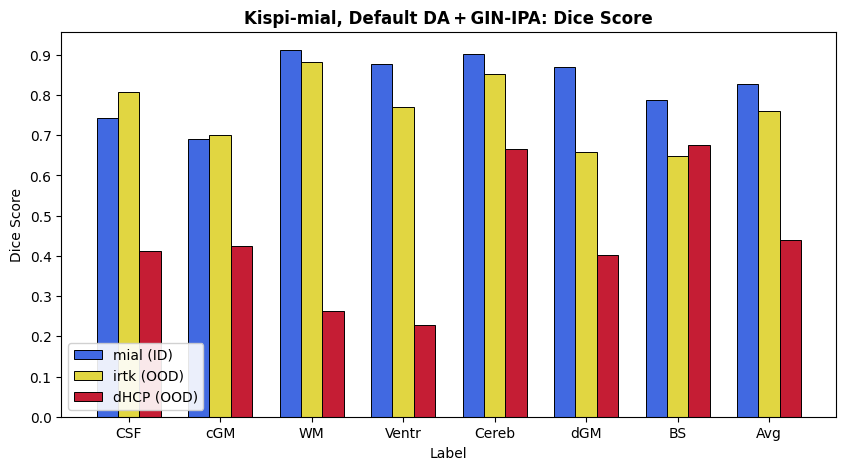
\includegraphics[width=0.8\textwidth]{figures/mial_both_DC.png} \\
  \vspace{10pt}
  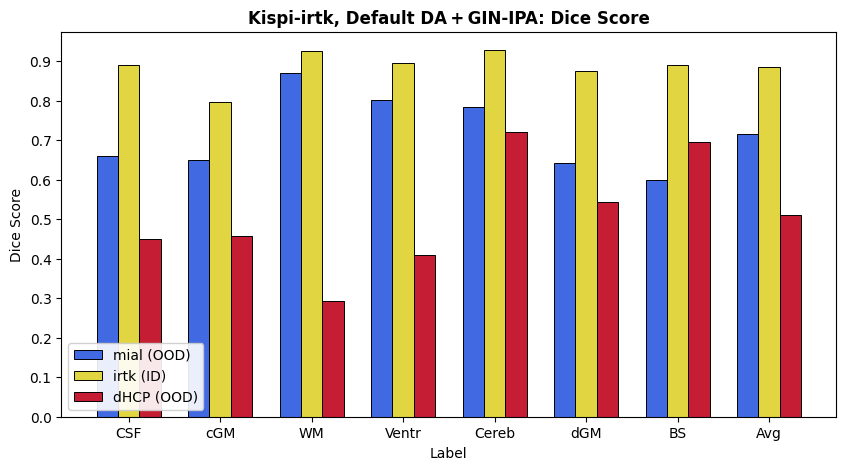
\includegraphics[width=0.8\textwidth]{figures/irtk_both_DC.png} \\
  \vspace{10pt}
  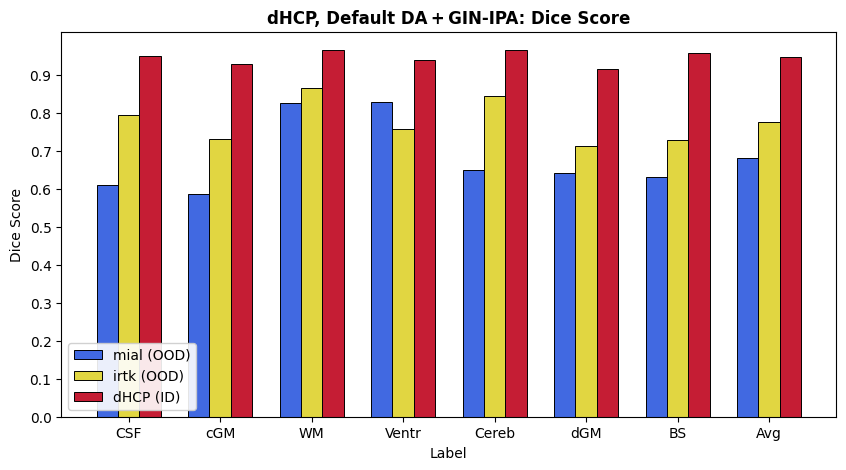
\includegraphics[width=0.8\textwidth]{figures/dHCP_both_DC.png}
  \caption{Dice score across datasets and labels for the combined DA (default\,+\,GIN-IPA) model. From top to bottom: training on Kispi-mial, on Kispi-irtk, and on dHCP.}
  \label{fig:both_DC}
\end{figure}

\section{Comparison of Model Performances} \label{sec:ComparisonOfModelPerformances}
In order to assess the relative contribution of the proposed augmentation strategies, two sets of comparisons between the models were designed:
\begin{itemize}
  \item the nnU-Net baseline with default data augmentation versus the GIN-IPA DA model
  \item the GIN-IPA DA model versus the combined strategy including both default and GIN-IPA augmentations
\end{itemize}
The distributions of each of the three evaluation metrics---DSC, VS, and HD95---were analyzed, at the level of individual tissues, and globally, involving all the labels.

Kernel density estimation (KDE) plots were generated for each metric and label, separately for the two model pairs under comparison. Beyond visual inspection, statistical analyses were employed to quantify the significance and magnitude of the observed differences. The Wilcoxon signed-rank test was used to test the null hypothesis of equal paired performance between models. Corresponding \textit{p}-values were computed to assess whether the proposed augmentation strategy led to statistically significant improvements. Besides, Cohen's \textit{d} was computed to quantify the magnitude of the improvement. Following conventional thresholds, \numlist{0.2; 0.5; 0.8} correspond to small, medium, and large effects, respectively. See Section \ref{sec:StatisticalPerformanceAssessment} for more details about the aforementioned tools. Tables with the complete statistical results are reported in Appendix \hyperref[app:SupplementaryTables]{B} (Tabs.\,\ref{tab:baseline_vs_ginipa_stats}, \ref{tab:ginipa_vs_combined_stats}).

\paragraph{Baseline vs.\ GIN-IPA}
\begin{itemize}
  \item \textbf{Train on Kispi-mial}
  \begin{itemize}
    \item \textbf{Inference on Kispi-mial:} no difference in performance.
    \item \textbf{Inference on Kispi-irtk:} CSF improves in DSC (\numrange[range-open-phrase=from\ ]{0.77}{0.81}, $\abs{d}=0.2$), VS (\numrange[range-open-phrase=from\ ]{-0.17}{-0.2}, $\abs{d}=0.6$), and HD95 (\numrange[range-open-phrase=from\ ]{3.4}{2.6}, $\abs{d}=0.2$); ventricles slightly improve in DSC (\numrange[range-open-phrase=from\ ]{0.74}{0.77}, $\abs{d}=0.3$) and HD95 (\numrange[range-open-phrase=from\ ]{3.5}{1.5}, $\abs{d}=0.4$). These improvements are due to a performance improvement of the GIN-IPA model on volumes that were poorly-segmented by the baseline model (see Fig.\,\ref{fig:1_mial_irtk_ventr}) The same pattern is observed for other tissues (WM, cerebellum).
    \item \textbf{Inference on dHCP:} significant, strong improvements in DSC and VS for cGM (DSC: \numrange[range-open-phrase=from\ ]{0.36}{0.44}, VS: \numrange[range-open-phrase=from\ ]{-0.8}{-0.5}) and dGM (DSC: \numrange[range-open-phrase=from\ ]{0.20}{0.35}; VS: \numrange[range-open-phrase=from\ ]{-1.6}{-1.3}). The corresponding KDE plots are in Fig.\,\ref{fig:1_mial_dhcp_gm}. Overall, a small gain is observed (DSC: \numrange[range-open-phrase=from\ ]{0.40}{0.44}).
  \end{itemize}
  \item \textbf{Train on Kispi-irtk}
  \begin{itemize}
    \item \textbf{Inference on Kispi-mial:} significant, moderate improvements across DSC, VS, and HD95 for dGM (DSC: \numrange[range-open-phrase=from\ ]{0.71}{0.78}; VS: \numrange[range-open-phrase=from\ ]{0.9}{0.7}) and ventricles (DSC: \numrange[range-open-phrase=from\ ]{0.36}{0.44}; VS: \numrange[range-open-phrase=from\ ]{-0.5}{-0.2}). Small improvement overall (DSC: \numrange[range-open-phrase=from\ ]{0.63}{0.68}).
    \item \textbf{Inference on Kispi-irtk:} no difference in performance.
    \item \textbf{Inference on dHCP:} significant, strong improvements across all metrics and tissues. The mean DSC increases \numrange[range-open-phrase=from\ ]{0.34}{0.54} (see Tab.\,\ref{tab:1_irtk_dhcp_stats}). The KDE plots of DSC are in Fig.\,\ref{fig:1_irtk_dhcp_DC}, while the ones regarding VS and HD95 are reported in Appendix \hyperref[app:SupplementaryPlots]{A} (Figs.\,\ref{fig:1_irtk_dhcp_VS}, \ref{fig:1_irtk_dhcp_HD}).
  \end{itemize}
  \item \textbf{Train on dHCP}
  No differences observed on any inference dataset, metric, or label.
\end{itemize}

\begin{figure}[htbp]
  \centering
  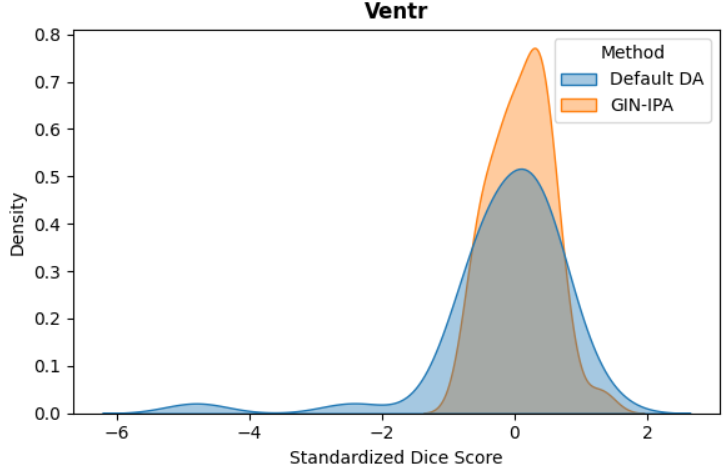
\includegraphics[width=0.45\textwidth]{figures/1_mial-irtk_DC_Ventr.png}\quad
  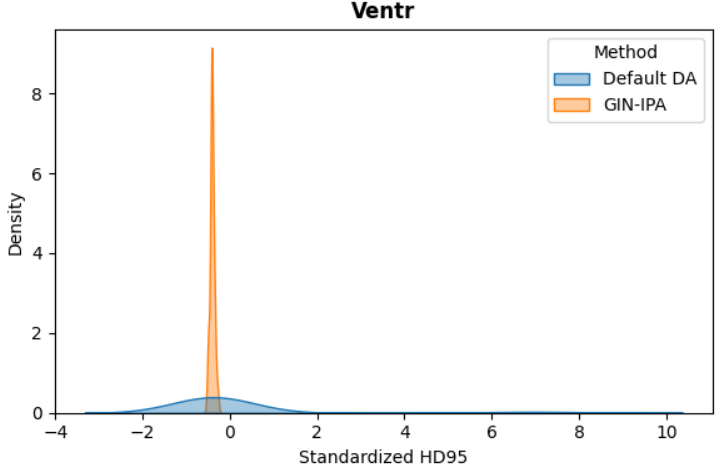
\includegraphics[width=0.45\textwidth]{figures/1_mial-irtk_HD_Ventr.png}
  \caption{Baseline vs.\ GIN-IPA: KDE plots of DSC (left) and HD95 (right) in ventricles, from models trained on Kispi-mial and inferring on Kispi-irtk.}
  \label{fig:1_mial_irtk_ventr}
\end{figure}

\begin{figure}[htbp]
  \centering
  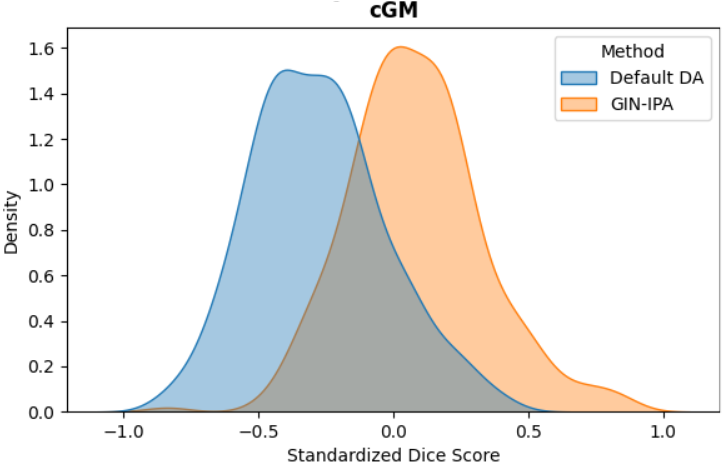
\includegraphics[width=0.45\textwidth]{figures/1_mial-dhcp_DC_cGM.png}\quad
  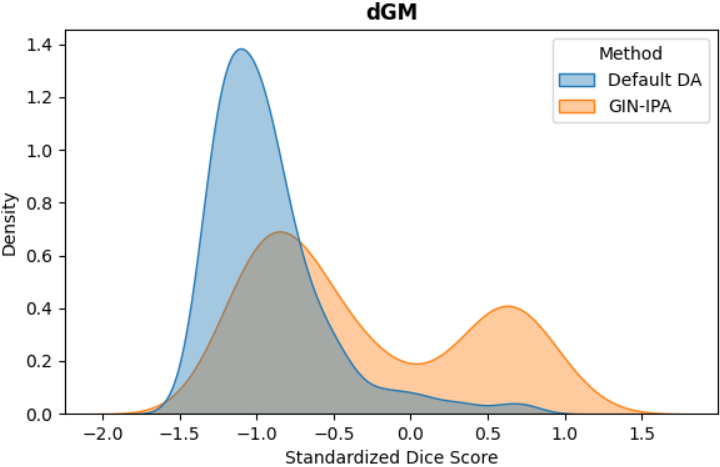
\includegraphics[width=0.46\textwidth]{figures/1_mial-dhcp_DC_dGM.png} \\
  \vspace{10pt}
  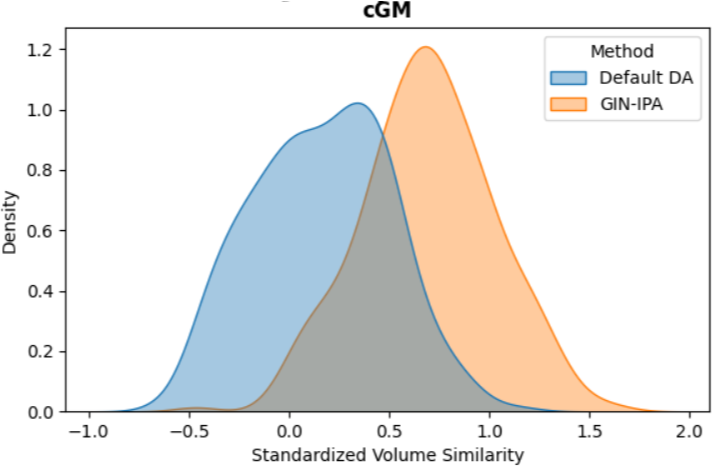
\includegraphics[width=0.45\textwidth]{figures/1_mial-dhcp_VS_cGM.png}\quad
  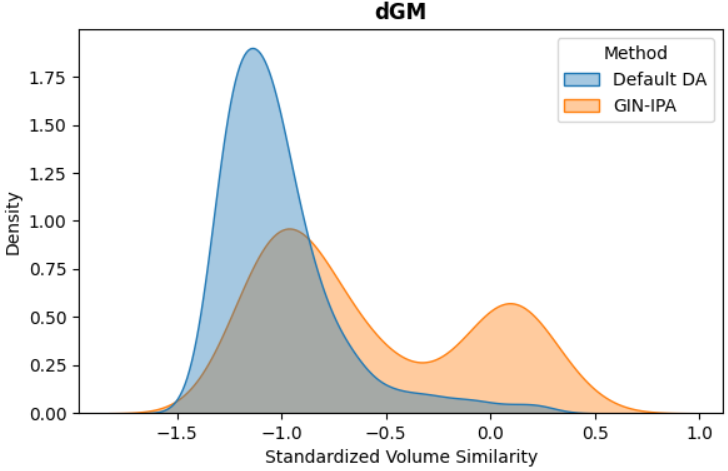
\includegraphics[width=0.46\textwidth]{figures/1_mial-dhcp_VS_dGM.png}
  \caption{Baseline vs.\ GIN-IPA: KDE plots of DSC (top) and VS (bottom) in cortical gray matter and deep gray matter, from models trained on Kispi-mial and inferring on dHCP.}
  \label{fig:1_mial_dhcp_gm}
\end{figure}

\begin{figure}[htbp]
  \centering
  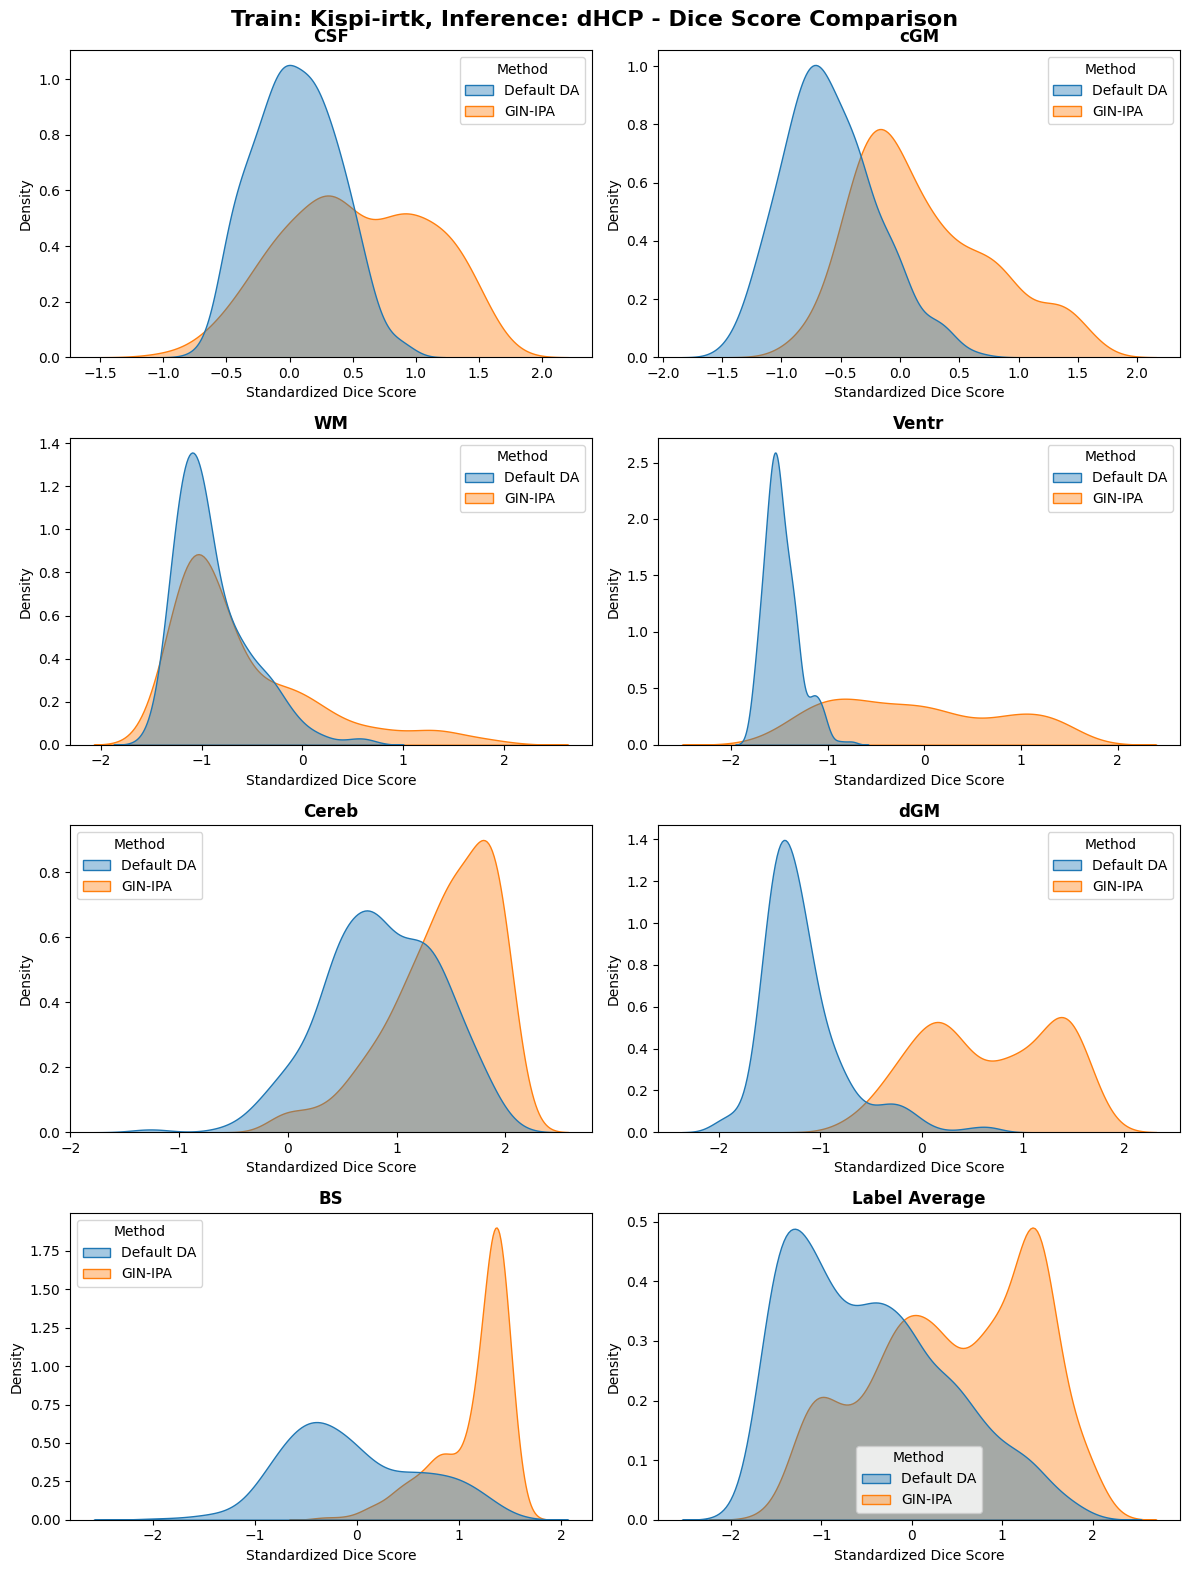
\includegraphics[width=0.95\textwidth]{figures/1_irtk-dhcp_DC.png}
  \caption{Baseline vs.\ GIN-IPA: KDE plots of DSC across each label and globally, from models trained on Kispi-irtk and inferring on dHCP.}
  \label{fig:1_irtk_dhcp_DC}
\end{figure}

\begin{table}[htbp]
  \centering
  \begin{tabular}{c|c|c|c}
    \toprule
    \textbf{Metric} & \textbf{Label} & \makecell{\textbf{Mean perf.} \\ \textbf{variation}} & \textbf{Cohen's |\textit{d}|} \\
    \midrule
    \multirow{8}{*}{\makecell{DSC \\ $(\times 10^{-2})$}}
      & CSF & $45 \rightarrow 56$ & $1.0$ \\
      & cGM & $31 \rightarrow 48$ & $1.6$ \\
      & WM & $24 \rightarrow 30$ & $0.5$ \\
      & Ventr. & $11 \rightarrow 42$ & $2.2$ \\
      & Cereb. & $63 \rightarrow 76$ & $1.1$ \\
      & dGM & $18 \rightarrow 59$ & $3.4$ \\
      & BS & $43 \rightarrow 70$ & $2.3$ \\
      & \textbf{Total} & $34 \rightarrow 54$ & $1.1$ \\
    \hline
    \multirow{8}{*}{VS}
      & CSF & $1.0 \rightarrow 0.7$ & $1.5$ \\
      & cGM & $1.1 \rightarrow 0.7$ & $1.6$ \\
      & WM & $1.4 \rightarrow 1.3$ & $0.4$ \\
      & Ventr. & $1.8 \rightarrow 1.1$ & $2.2$ \\
      & Cereb. & $0.3 \rightarrow 0.1$ & $0.5$ \\
      & dGM & $1.4 \rightarrow 0.6$ & $2.0$ \\
      & BS & $0.8 \rightarrow 0.4$ & $1.4$ \\
      & \textbf{Total} & $1.1 \rightarrow 0.7$ & $0.8$ \\
    \hline
    \multirow{8}{*}{HD95}
      & CSF & $35 \rightarrow 32$ & $0.3$ \\
      & cGM & $40 \rightarrow 37$ & $0.3$ \\
      & WM\textsuperscript{*} & $42 \rightarrow 42$ & $0.1$ \\
      & Ventr. & $48 \rightarrow 44$ & $0.3$ \\
      & Cereb. & $55 \rightarrow 44$ & $0.6$ \\
      & dGM & $57 \rightarrow 37$ & $1.1$ \\
      & BS & $64 \rightarrow 30$ & $1.4$ \\
      & \textbf{Total} & $49 \rightarrow 38$ & $0.6$ \\
    \bottomrule
  \end{tabular}
  \caption{Baseline vs.\ GIN-IPA: mean performance variation and Cohen's |\textit{d}| across metrics and labels, from models trained on Kispi-irtk and inferring on dHCP. To enhance comprehensibility, the absolute value of VS is shown. The variation of HD95 in WM---marked by the asterisk---is the only one that is not statistically significant (\textit{p}-value $< 0.01$).}
  \label{tab:1_irtk_dhcp_stats}
\end{table}

\paragraph{GIN-IPA vs.\ Combined Augmentation}
\begin{itemize}
  \item \textbf{Train on Kispi-mial}
  \begin{itemize}
    \item \textbf{Inference on Kispi-mial:} no difference in performance.
    \item \textbf{Inference on Kispi-irtk:} no difference in performance.
    \item \textbf{Inference on dHCP:} small improvements across DSC, VS, and HD95 for ventricles (DSC: \numrange[range-open-phrase=from\ ]{0.18}{0.23}, $\abs{d}=0.3$) and dGM (DSC: \numrange[range-open-phrase=from\ ]{0.35}{0.40}, $\abs{d}=0.3$).% The corresponding KDE plots are in Fig.\,\ref{fig:2_mial_dhcp_DC}.
  \end{itemize}
  \item \textbf{Train on Kispi-irtk}
  \begin{itemize}
    \item \textbf{Inference on Kispi-mial:} moderate improvements (see Fig.\,\ref{fig:2_irtk_mial}) in DSC and HD95 for cGM (DSC: \numrange[range-open-phrase=from\ ]{0.59}{0.65}; HD95: \numrange[range-open-phrase=from\ ]{2.2}{1.7}) and cerebellum (DSC: \numrange[range-open-phrase=from\ ]{0.73}{0.78}; HD95: \numrange[range-open-phrase=from\ ]{4.8}{2.3}). Small improvement overall.
    \item \textbf{Inference on Kispi-irtk:} no difference in performance.
    \item \textbf{Inference on dHCP:} combined augmentation performs significantly worse than GIN-IPA alone, especially for CSF, cerebellum, and dGM across all the metrics.
  \end{itemize}
  \item \textbf{Train on dHCP}
  No differences observed on any inference dataset, metric, or label.
\end{itemize}

\comment{
\begin{figure}[p]
  \centering
  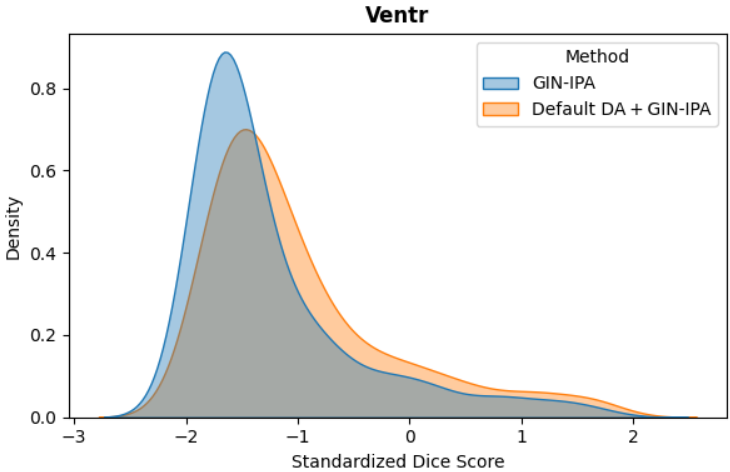
\includegraphics[width=0.445\textwidth]{figures/2_mial-dhcp_DC_Ventr.png}\quad
  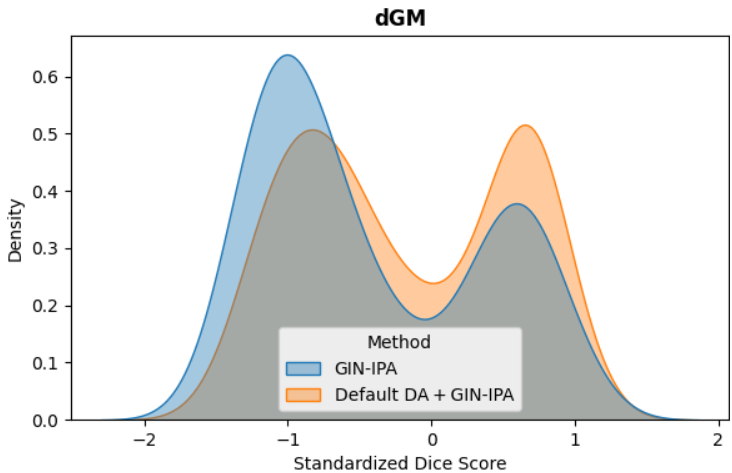
\includegraphics[width=0.45\textwidth]{figures/2_mial-dhcp_DC_dGM.png}
  \caption{GIN-IPA vs.\ combined DA: KDE plots of DSC in ventricles and deep gray matter, from models trained on Kispi-mial and inferring on dHCP.}
  \label{fig:2_mial_dhcp_DC}
\end{figure}
}

\begin{figure}[htbp]
  \centering
  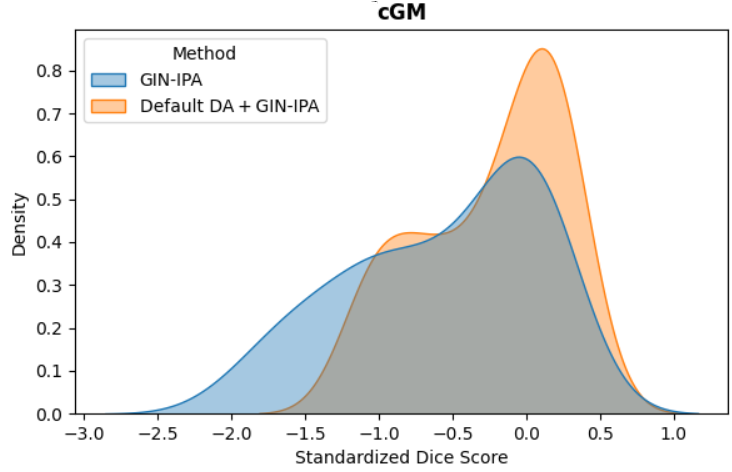
\includegraphics[width=0.45\textwidth]{figures/2_irtk-mial_DC_cGM.png}\quad
  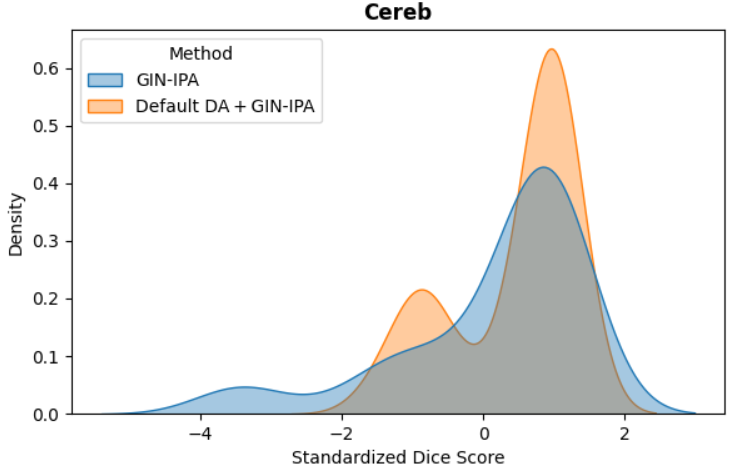
\includegraphics[width=0.45\textwidth]{figures/2_irtk-mial_DC_Cereb.png} \\
  \vspace{10pt}
  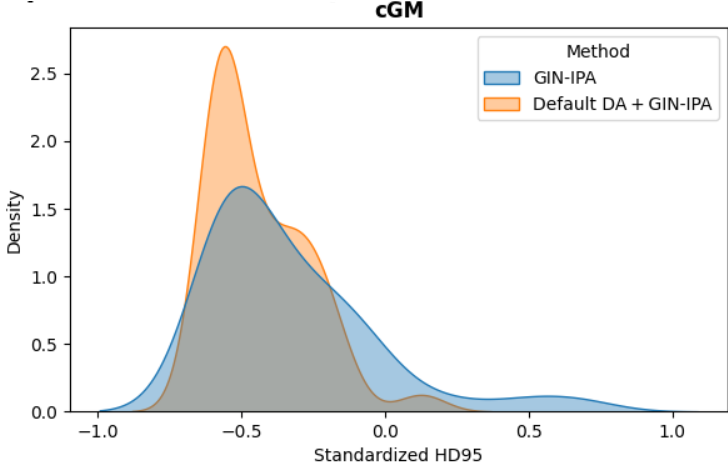
\includegraphics[width=0.45\textwidth]{figures/2_irtk-mial_HD_cGM.png}\quad
  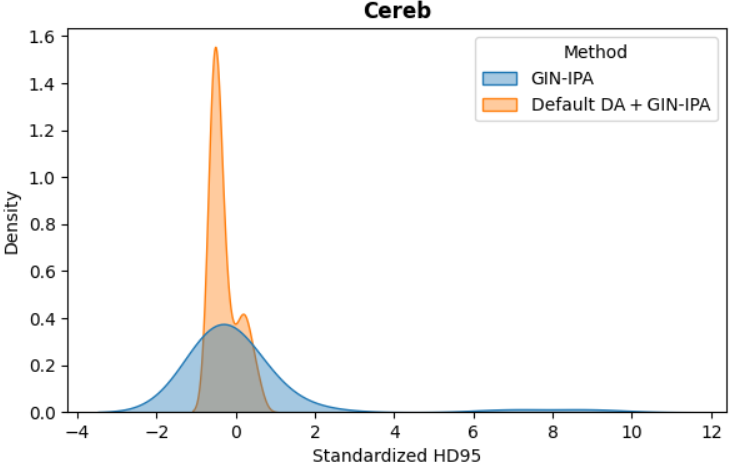
\includegraphics[width=0.45\textwidth]{figures/2_irtk-mial_HD_Cereb.png}
  \caption{GIN-IPA vs.\ combined DA: KDE plots of DSC (top) and HD (bottom) in cortical gray matter and cerebellum, from models trained on Kispi-irtk and inferring on Kispi-mial.}
  \label{fig:2_irtk_mial}
\end{figure}

\section{Performance by Pathology} \label{sec:PerformanceByPathology}
Since dHCP only includes healthy scans, it can be interesting to investigate how the data augmentation methods behave when stratification on subject health is taken into account. Hence, the performance of the models was analyzed separately for healthy and pathological cases, in order to isolate the effect of brain abnormalities on segmentation accuracy.

The plots below (Fig.\,\ref{fig:pathology_summary_1} and Fig.\,\ref{fig:pathology_summary_2}) are relative to models trained on dHCP and separately tested on healthy and pathological cases in Kispi-mial and Kispi-irtk. Metrics relative to the test set of dHCP are shown as a reference. The difference between neurotypical and pathological cases is evident but not dramatic for all metrics---volume similarity shows a delta which is especially small. Neither GIN-IPA nor the combined DA help at increasing any metric in neurotypical subjects. For the pathological cases, GIN-IPA produces a small improvement in all metrics with respect to the baseline model, while performs equivalent to the combined DA model. It is also interesting to notice that, despite the difference in image quality claimed in \cite{FeTA2021_review}, the performance of the model trained on dHCP is equivalent when inferring on healthy Kispi-mial and Kispi-irtk. On the other hand, a performance difference is observed when inferring on pathological Kispi-mial and Kispi-irtk cases. This suggests that the low-quality images are mainly among the pathological cases.

\begin{figure}[htbp]
  \centering
  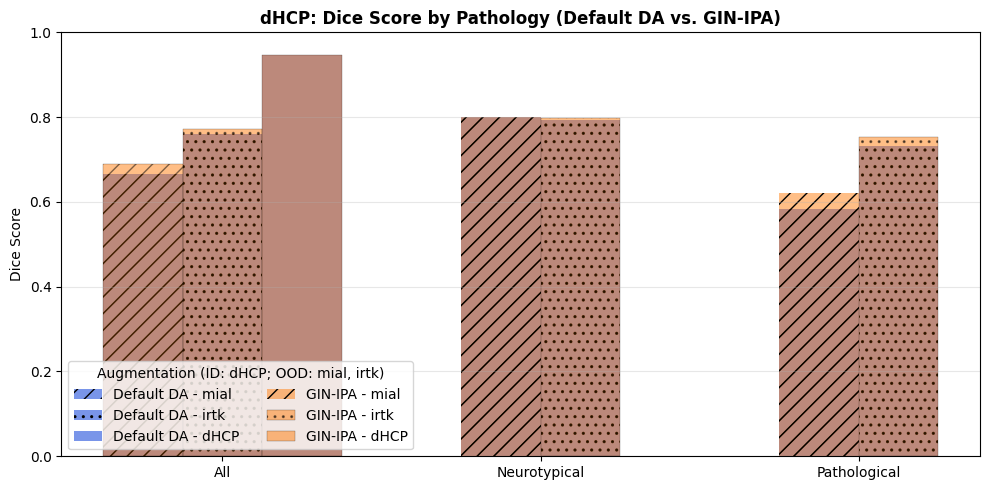
\includegraphics[width=0.85\textwidth]{figures/1_pathology_DC.png} \\
  \vspace{10pt}
  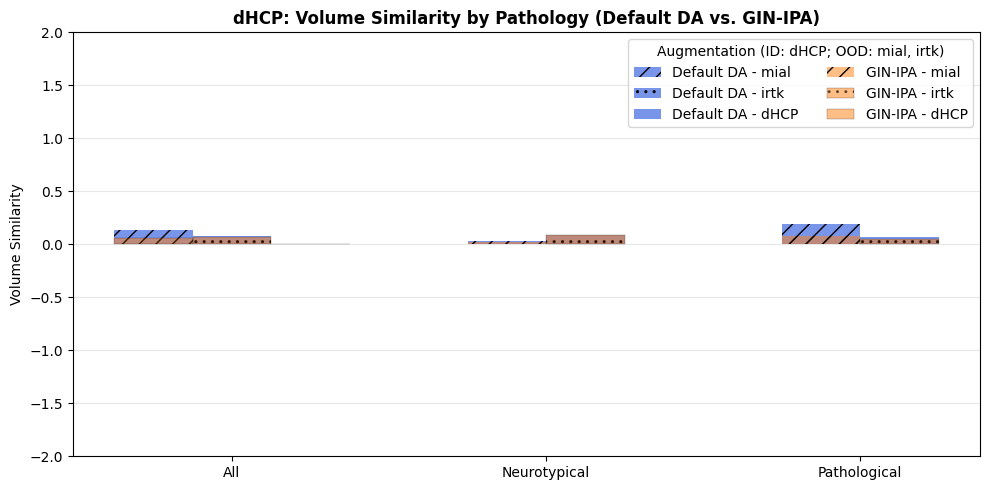
\includegraphics[width=0.85\textwidth]{figures/1_pathology_VS.png} \\
  \vspace{10pt}
  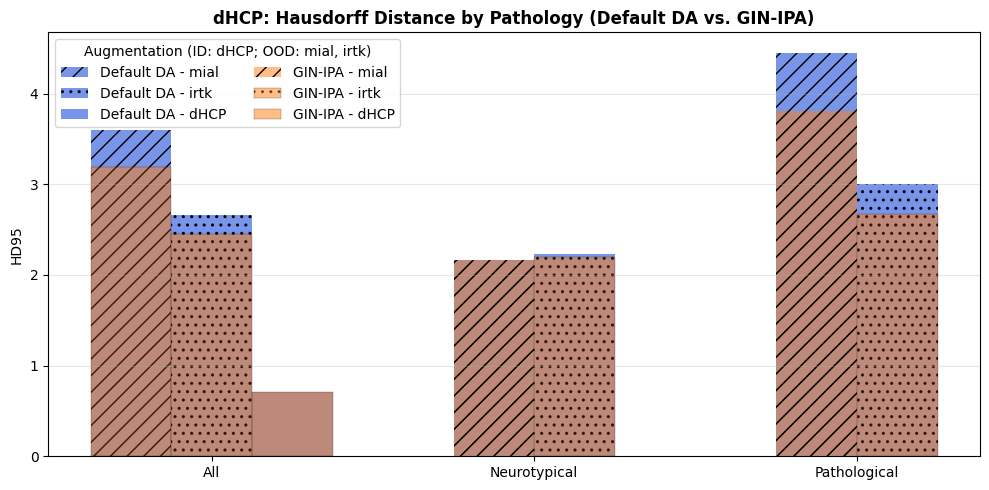
\includegraphics[width=0.85\textwidth]{figures/1_pathology_HD.png}
  \caption{Comparison of the segmentation performance by pathology, between the baseline and the GIN-IPA augmentation models. From top to bottom: Dice score, volume similarity, and Hausdorff distance 95\th percentile. Until the bars are brown, the metrics of the two models are equivalent.}
  \label{fig:pathology_summary_1}
\end{figure}

\begin{figure}[htbp]
  \centering
  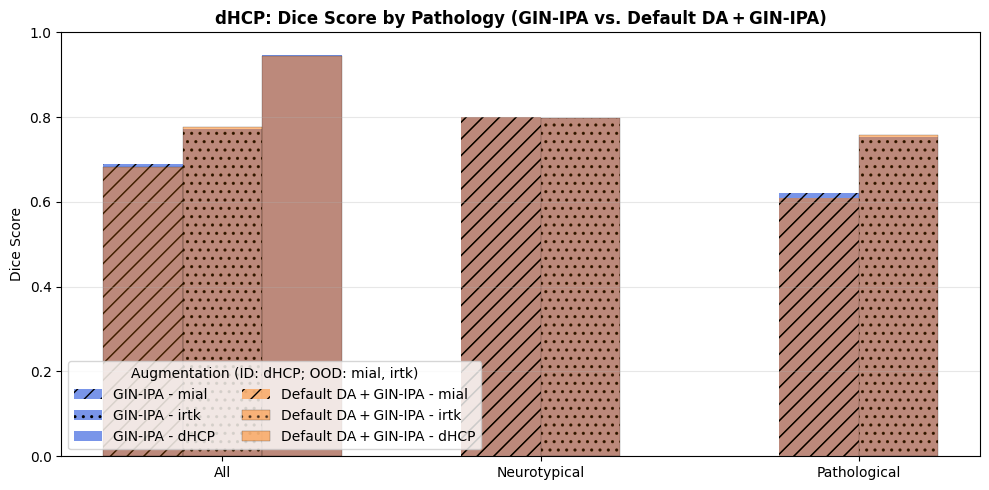
\includegraphics[width=0.85\textwidth]{figures/2_pathology_DC.png} \\
  \vspace{10pt}
  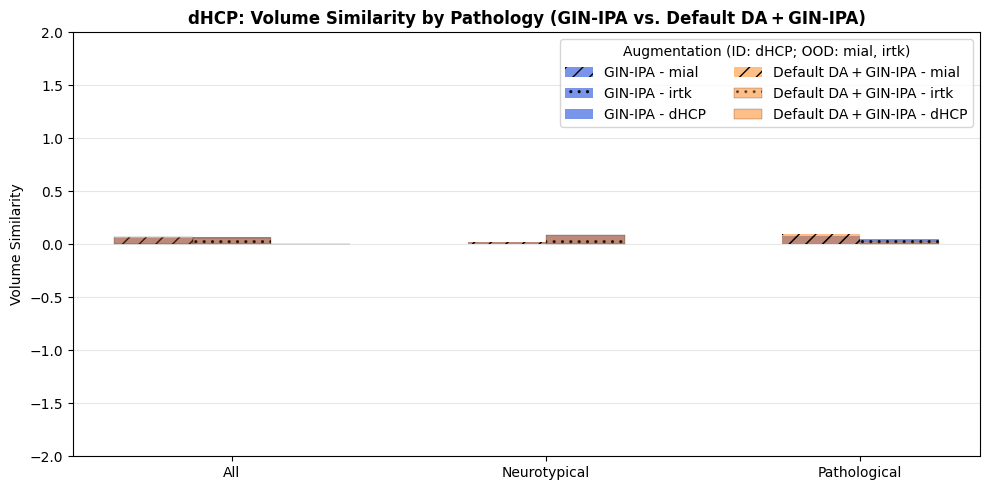
\includegraphics[width=0.85\textwidth]{figures/2_pathology_VS.png} \\
  \vspace{10pt}
  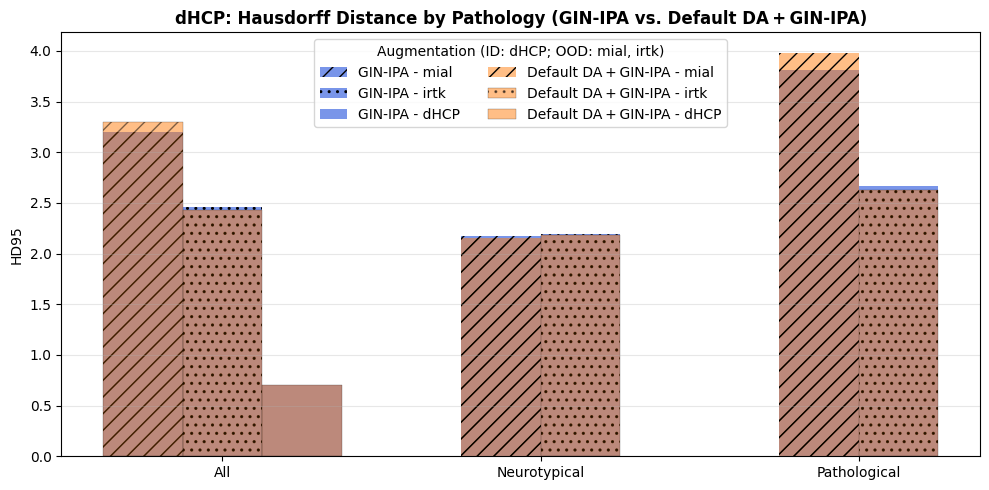
\includegraphics[width=0.85\textwidth]{figures/2_pathology_HD.png}
  \caption{Comparison of the segmentation performance by pathology, between the GIN-IPA and the combined augmentation models. From top to bottom: Dice score, volume similarity, and Hausdorff distance 95\th percentile. Until the bars are brown, the metrics of the two models are equivalent.}
  \label{fig:pathology_summary_2}
\end{figure}
